% debut d'un fichier latex standard
\documentclass[a4paper,12pt,twoside]{article}

% pour l'inclusion de figures en eps,pdf,jpg
\usepackage{graphicx}
\usepackage{subcaption}
\usepackage{wrapfig}
% quelques symboles mathematiques en plus
\usepackage{amsmath}
% le tout en langue francaise
%\usepackage[french]{babel}
% on peut ecrire directement les caracteres avec l'accent
% a utiliser sur Linux/Windows
\usepackage[utf8]{inputenc}
\usepackage[T1]{fontenc}
% a utiliser sur le Mac
%\usepackage[applemac]{inputenc}
% pour l'inclusion de links dans le document
\usepackage[colorlinks,bookmarks=false,linkcolor=blue,urlcolor=blue]{hyperref}
\usepackage{siunitx}
% pour les degrés
\usepackage{textcomp}
\paperheight=297mm
\paperwidth=210mm

\setlength{\textheight}{235mm}
\setlength{\topmargin}{-1.2cm} % pour centrer la page verticalement
%\setlength{\footskip}{5mm}
\setlength{\textwidth}{15cm}
\setlength{\oddsidemargin}{0.56cm}
\setlength{\evensidemargin}{0.56cm}

\pagestyle{plain}

% quelques abreviations utiles
\def \be {\begin{equation}}
\def \ee {\end{equation}}
\def \dd  {{\rm d}}

\newcommand{\mail}[1]{{\href{mailto:#1}{#1}}}
\newcommand{\ftplink}[1]{{\href{ftp://#1}{#1}}}
%
% latex SqueletteRapport.tex      % compile la source LaTeX
% xdvi SqueletteRapport.dvi &     % visualise le resultat
% dvips -t a4 -o SqueletteRapport.ps SqueletteRapport % produit un PostScript
% ps2pdf SqueletteRapport.ps      % convertit en pdf

% pdflatex SqueletteRapport.pdf    % compile et produit un pdf

% ======= Le document commence ici ======

\begin{document}
% Le titre, l'auteur et la date
\title{Heat problem\\{\small Physique Numérique I}\\{\small Rapport 5}}
\date{\today}
\author{Delphine Martres et Damien Korber\\{\small \mail{delphine.martres@epfl.ch} et \mail{damien.korber@epfl.ch}}}

\maketitle
\tableofcontents % Table des matieres


% Quelques options pour les espacements entre lignes, l'identation
% des nouveaux paragraphes, et l'espacement entre paragraphes
\baselineskip=16pt
\parindent=15pt
\parskip=5pt
\newpage


%%%% ON COMMENCE A ECRIRE D'ICI

\section{Introduction}

\begin{wrapfigure}{r}{0.55\textwidth}
 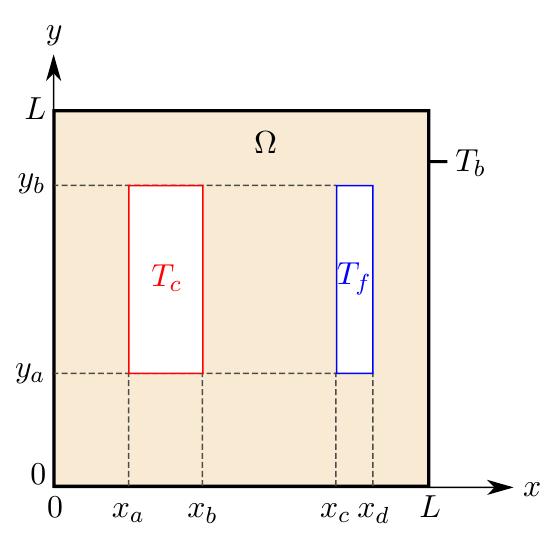
\includegraphics[width=0.45\textwidth]{graphs/schema.png}
 \caption{Geometry of the problem}
 \label{schema}
\end{wrapfigure}


This problem focuses on the propagation of heat in an homogeneous environment.
We consider two rectangular bodies of same height and respective temperatures $T_c = 200$°C and $T_f = -100$°C inside of a square box $\Omega$, of which the outside boundary is at Temperature $T_b = 0$°C. Initially, the temperature of the inside of the box is $T(t=0) = T_b$. The problems satisfies the heat equation \eqref{heateq}:

\begin{equation}
 \frac{\partial T}{\partial t} = D\nabla ^2 T
 \label{heateq}
\end{equation}
with $D=\kappa/(\rho C)=const$, where $\kappa=1.2~\si{\W \per \K \per \m}$ is the thermal conductivity, $\rho=1.2~\si{\kg \per \m^3}$ is the mass density, and $C=10^3~\si{\J \per \kg \per \K}$ is the specific heat capacity.


The geometry of the problem is as represented on Fig.\ref{schema}, where the parameters are: $L=10$ cm, $x_a=2$ cm, $x_b=4$ cm, $x_c=7.5$ cm, $x_d=8.5$ cm, $y_a=3$ cm, and $y_b=8$ cm. Numerically, the system is discretized as a $N\times N$ regular grid.

In this report, the evolution of the system with respect to time will be simulated in order to study the heat flux and thermal power of each body. The simulation is done using the Jacobi method.

% TODO : Explication de la dérivation spatiale. (laplacien, ...)

\section{Convergence and stability}

A convergence study of the temperature with the time step $\Delta t$ was made for $N=40$ (Fig.\ref{fig:b-conv40}) and $N=80$ (Fig.\ref{fig:b-conv80}) at the center point (0.05,0.05) of the system using linear interpolation. In both cases the convergence seems linear, as expected from the Jacobi algorithm. %TODO : why ?

\begin{figure}[h]
  \centering
  \begin{subfigure}[t]{0.45\textwidth}
    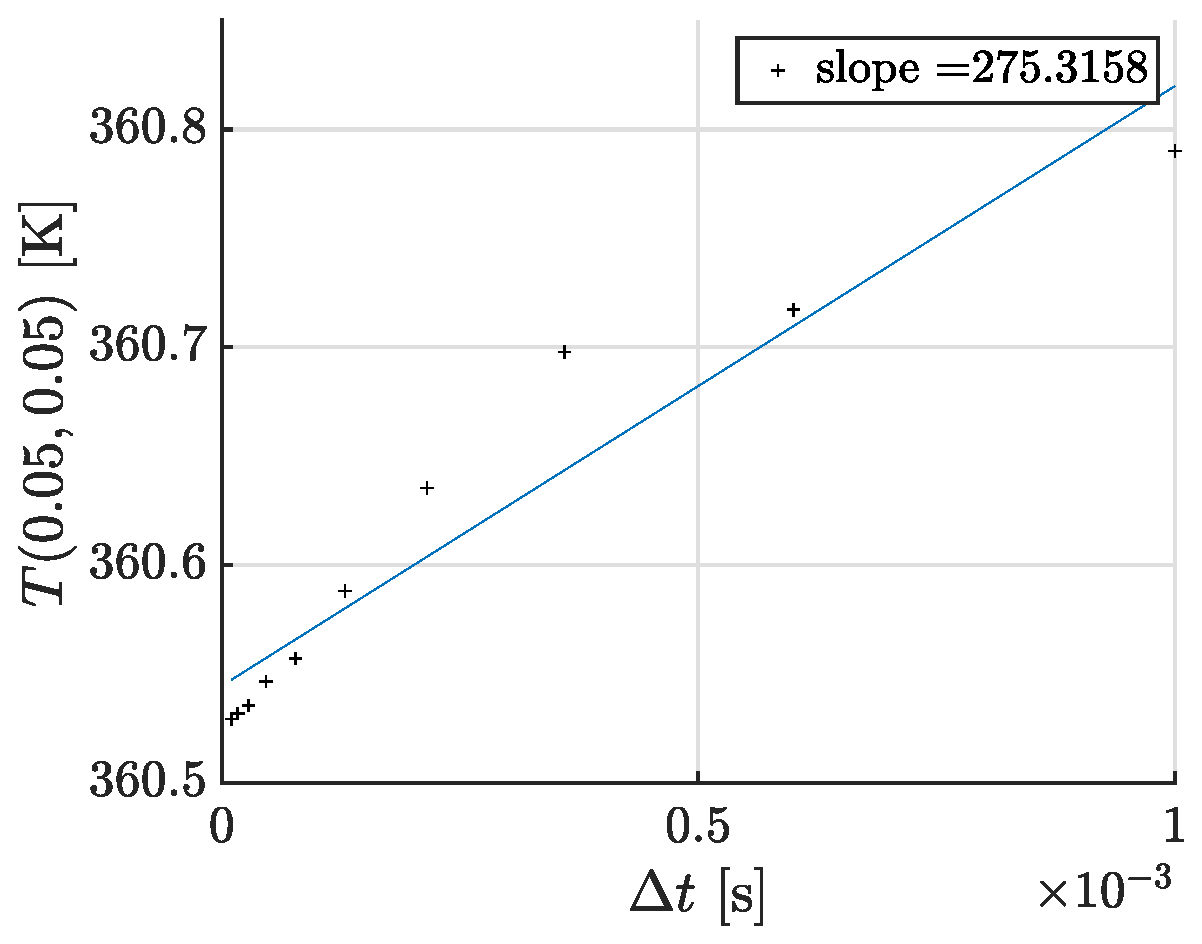
\includegraphics[width=\textwidth]{graphs/b_conv40.eps}

    \caption{N=40}
    \label{fig:b-conv40}
  \end{subfigure}
  ~
  \begin{subfigure}[t]{0.45\textwidth}
    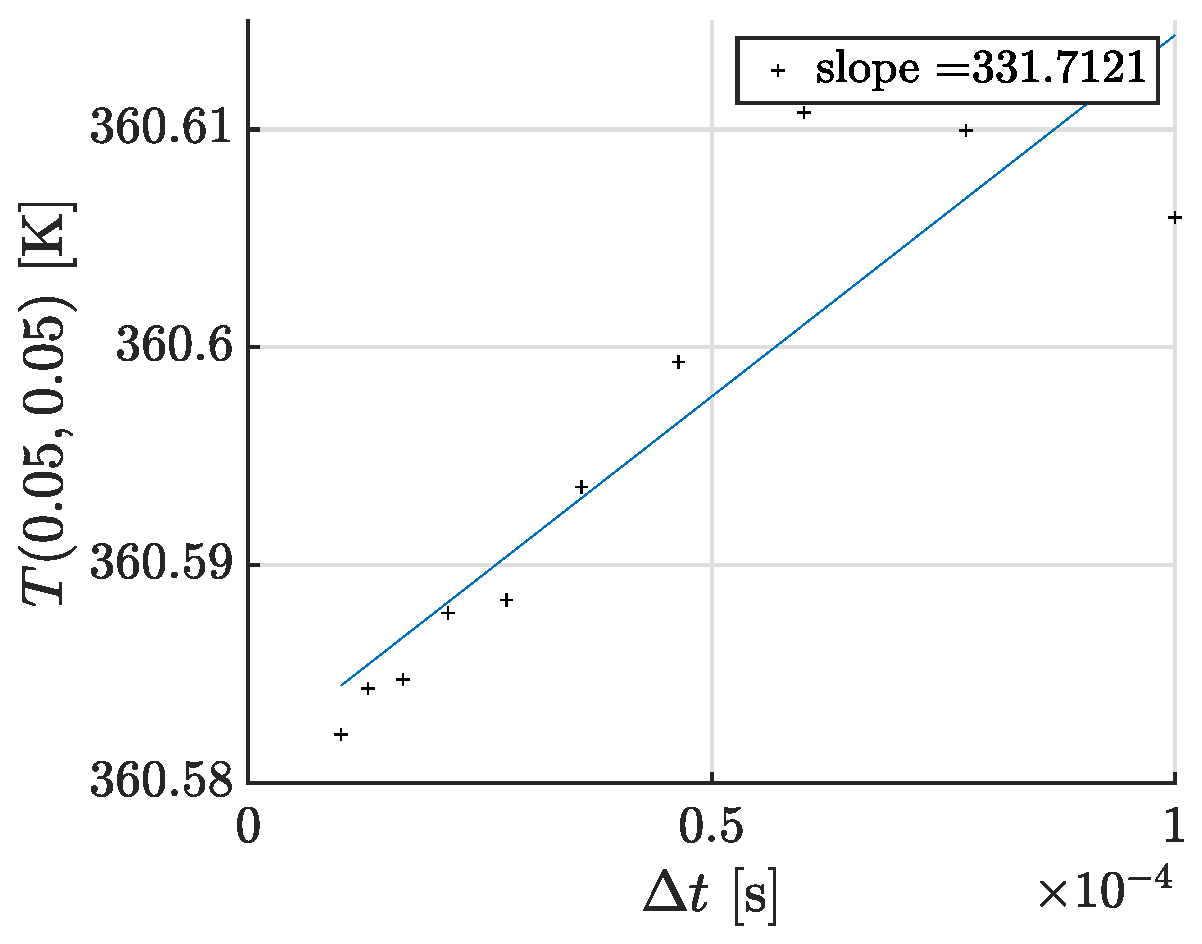
\includegraphics[width=\textwidth]{graphs/b_conv80.eps}
    \caption{N=80}
    \label{fig:b-conv80}
  \end{subfigure}
  \caption{Convergence study of the temperature for a varying $\Delta t$}
  \label{fig:bconv}
\end{figure}

The limit of stability in function of $\Delta t$ was also studied in both cases on Fig.\ref{fig:blim}. The limit of stability for $N=40$ is about $\Delta t = 1.61 \cdot 10^{-3}$ s, while the limit for $N=80$ is around $\Delta t = 3.95 \cdot 10^{-4}$ s. Thus we can observe that while a higher $N$ allows for better precision on the computed values, it has a much lower limit of stability. Using this information, all of the following simulations will be run using $N=40$ and a time step $\Delta t = 1\cdot 10^{-4}$.

\begin{figure}[h]
  \centering
  \begin{subfigure}[t]{0.45\textwidth}
    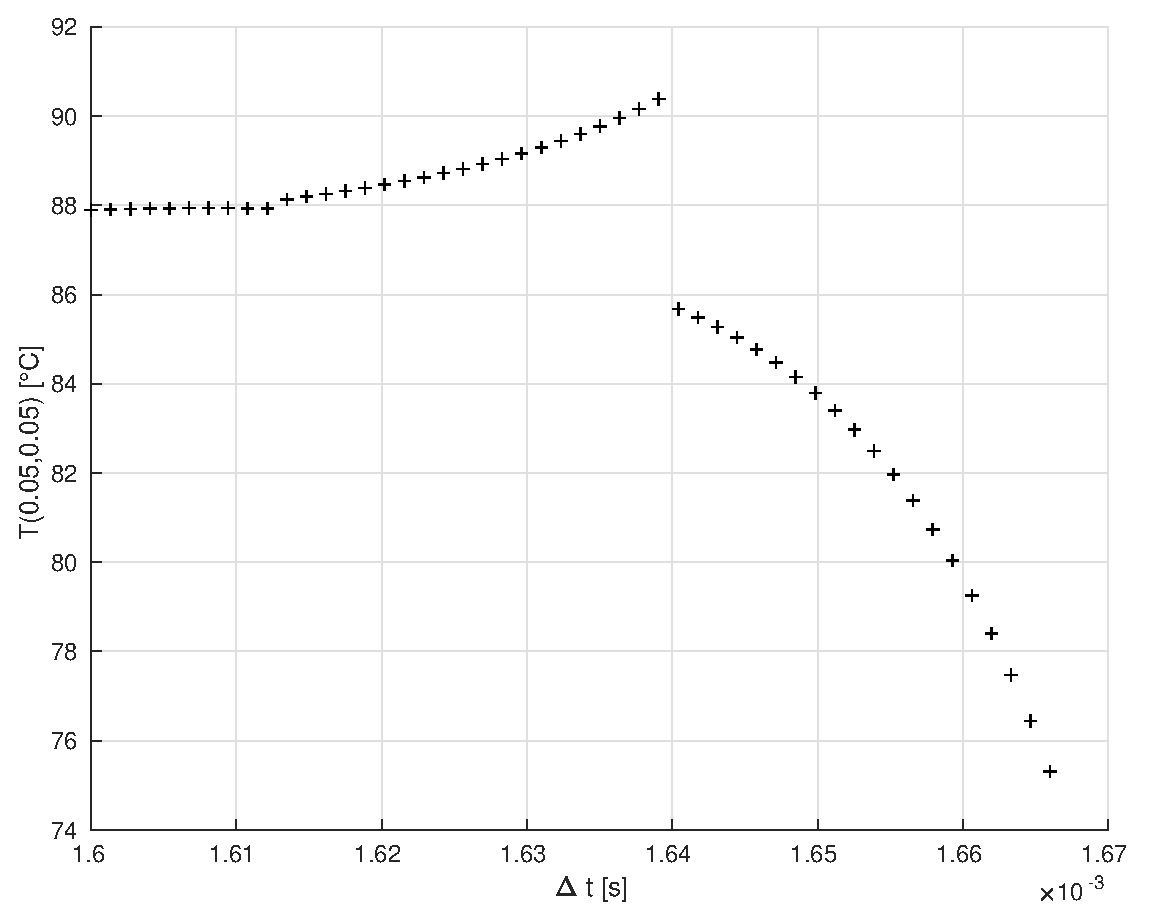
\includegraphics[width=\textwidth]{graphs/b_lim40.eps}

    \caption{N=40}
    \label{fig:b-lim40}
  \end{subfigure}
  ~
  \begin{subfigure}[t]{0.45\textwidth}
    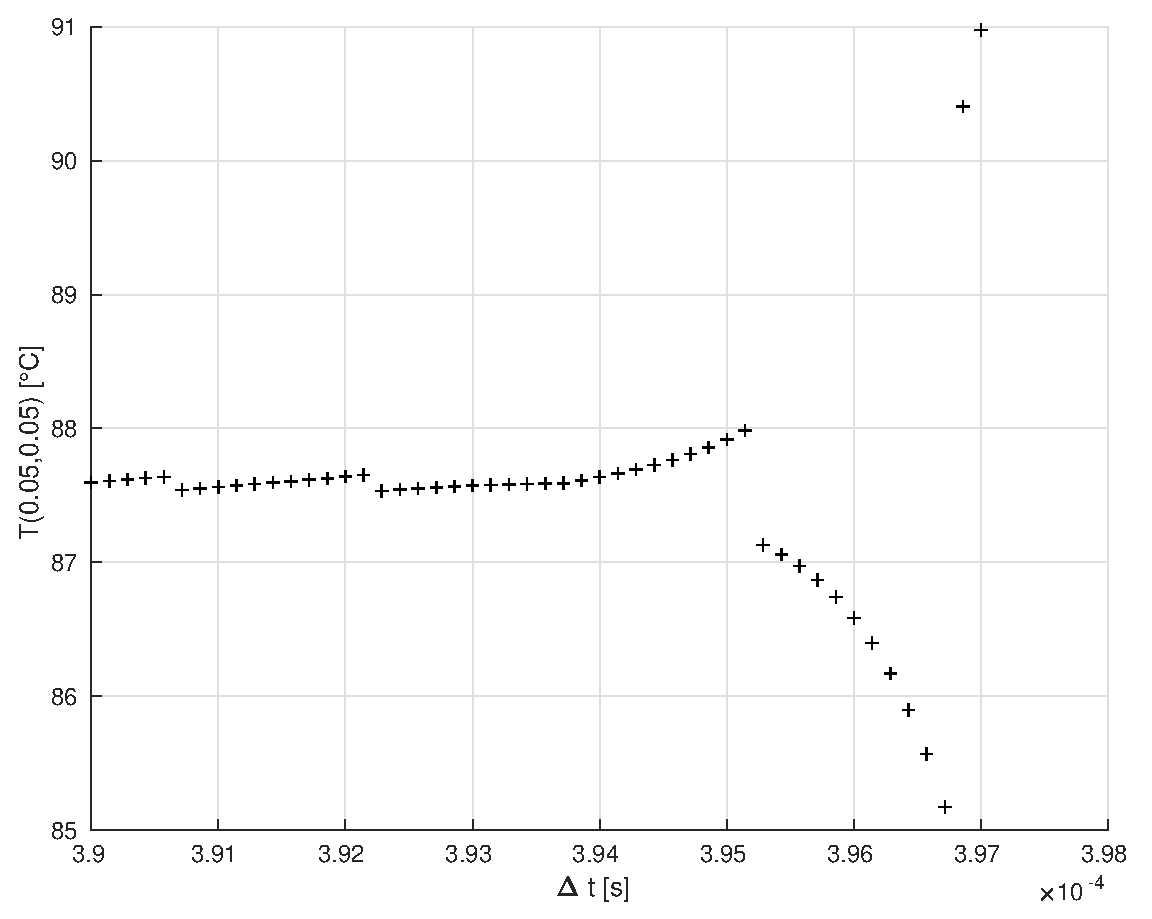
\includegraphics[width=\textwidth]{graphs/b_lim80.eps}
    \caption{N=80}
    \label{fig:b-lim80}
  \end{subfigure}
  \caption{Limit of stability in $\Delta t$}
  \label{fig:blim}
\end{figure}

\section{Heat flux}
This section focuses on the analysis of the behavious of the heat flux.
The heat flux is obtained with equation \eqref{eq:flux-chaleur}.

\begin{equation}
  \vec{j} = -\kappa\vec{\nabla} T
  \label{eq:flux-chaleur}
\end{equation}

where $\kappa$ is the thermal conductivity.
By using a forward finite difference method, $\vec{j}$ can be numerically computed using equation \eqref{eq:flux-chaleur-numerique}.

\begin{equation}
  \vec{j} = -\frac{\kappa}{h}
  \begin{pmatrix}
    T^k_{i+1,j} - T^k_{i,j} & T^k_{i,j+1} - T^k_{i,j}
  \end{pmatrix}
  \label{eq:flux-chaleur-numerique}
\end{equation}

At $t=\SI{0.1}{\s}$, with a stable $\Delta t$ and $N=40$, the flux heat can be seen in two ways, depending on the interest.
On figure \ref{fig:c-temp}, multiple information can be observed.
First, the temperature of the multiple points of the system can be studied using the color gradient.
These colors show the diffusion of heat through the homogeneous environment.
Next, the little arrows show the direction and the intensity of the heat flux.
As it can be observed, the heat flux goes from the hot source to a colder environment.
All of this can be explained by the second law of thermodynamics, which states that in a closed system, entropy never decreases. \cite{wiki:2nd-law}
Thus, the system wants to reach the thermodynamic equilibrum, and heat goes from hot to cold. %TODO : La dernière phrase est pas très belle.

% TODO : Idée - Faire le "spectre" de chaleur sur une bande horizontale.
% The result for the heat flux at $t=\SI{0.1}{\second}$ is given by figures \ref{fig:c-temp} and \ref{fig:c-heat-flux}.

\begin{figure}[h]
  \centering
  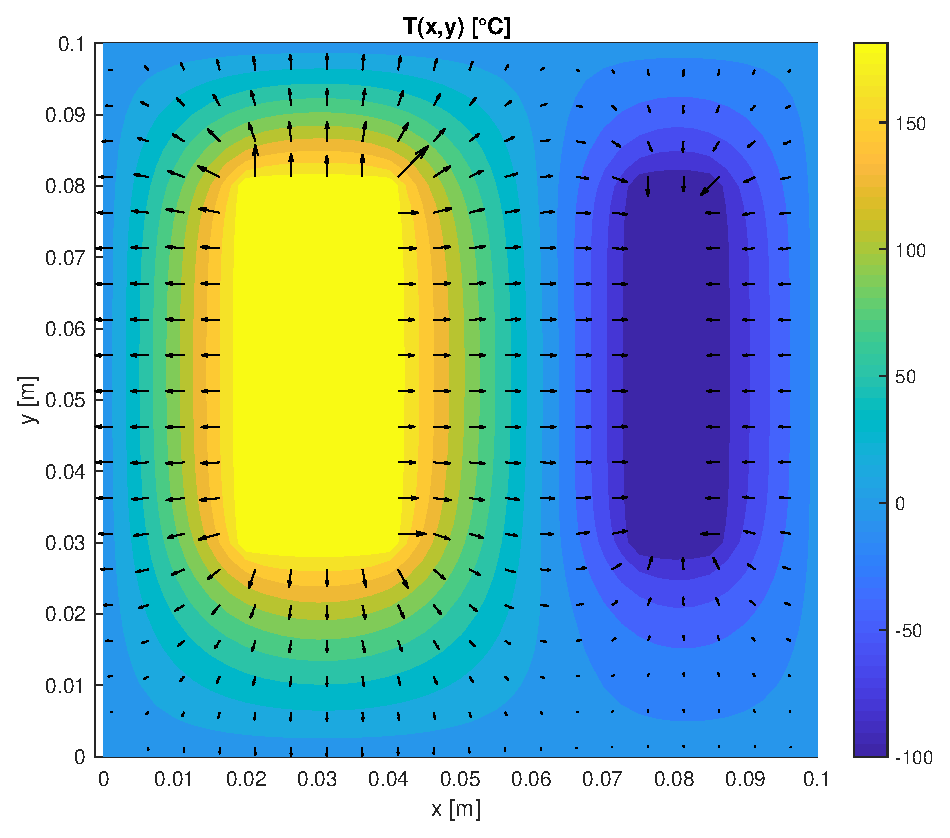
\includegraphics[width=0.6\textwidth]{graphs/c_temp.eps}
  \caption{Graph of temperatures at $t=\SI{0.1}{\s}$, represented by the color gradient, in Kelvin, with the direction and the intensity of the heat flux represented by the arrows.}
  \label{fig:c-temp}
\end{figure}

On figure \ref{fig:c-heat-flux}, the intensity of the heat flux can be observed using the color gradient.
The more yellow it gets, the higher the norm of the heat flux is. %TODO : Phrase pas très belle.
First, the graph shows indirectly the diffusion of heat through the environment.
When the intensity is lower, it either means that the environment is closer to thermodynamic equilibrum or that less heat is flowing. %TODO : Je sais pas si cette phrase a un intérêt, c'est évident.
But the most interesting point on this graph is the corners of the sources, in particular the hot source.
The majority of the environment has a norm for the heat flux around $\SI{10000}{\watt\per\square\meter}$. But on these corners, the norm of the heat flux reaches \SI{25000}{\watt\per\square\meter}.
This behavious does not appear on the border of the heat sources, so it is different from a simple "diffusion".
These are singularities. %TODO : C'est pas un peu fort.
This behavious can be compared to the the \textit{peak effect} \footnote{The name of this effect is directly translated from the french expression: \textit{effet de pointe}. No real translation of this effect in english seems to exist.}, an effect in electrostatics that describes the concentration of charges on the peak of a conductor.
This comparison is not innocent, as there is a mathematical similarity between the electric field and the heat flux.
The electric field $\vec{E}$ is derived from a scalar potential $\phi$, which give equation \eqref{eq:elec-field}.

\begin{equation}
  \vec{E} = \vec{\nabla}\phi
  \label{eq:elec-field}
\end{equation}

Equation \eqref{eq:elec-field} is similar to equation \eqref{eq:flux-chaleur}, as $\vec{j}$ is also derived from a scalar potential ($T$). %TODO : C'est juste de dire que T est un potentiel scalaire ?
Thus, the peaks in intensity on the corners of the sources can be compared to the \textit{peak effect} of electrostatics.

\begin{figure}[h]
  \centering
  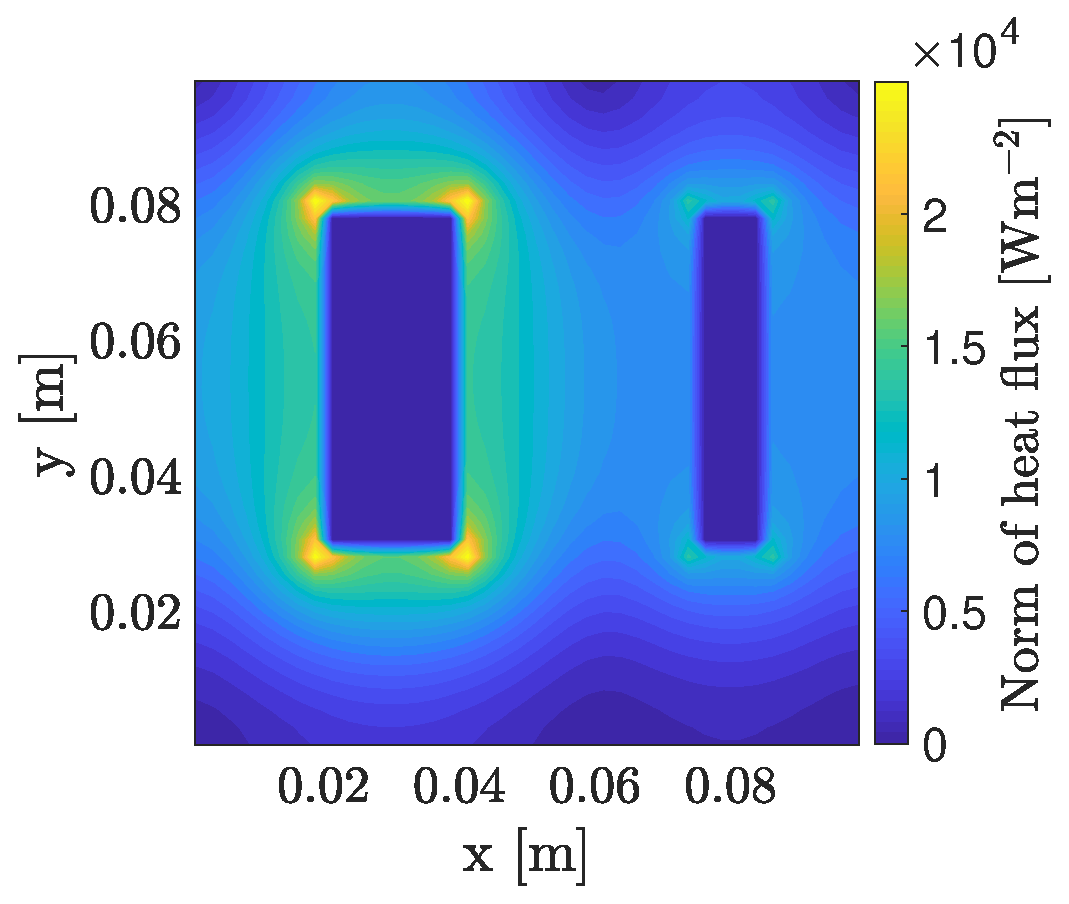
\includegraphics[width=0.6\textwidth]{graphs/c_heat_flux.eps}
  \caption{Intensity of the heat flux represented by the color gradient.}
  \label{fig:c-heat-flux}
\end{figure}
% \begin{figure}[h]
%   \centering
%   \begin{subfigure}[t]{0.45\textwidth}
%     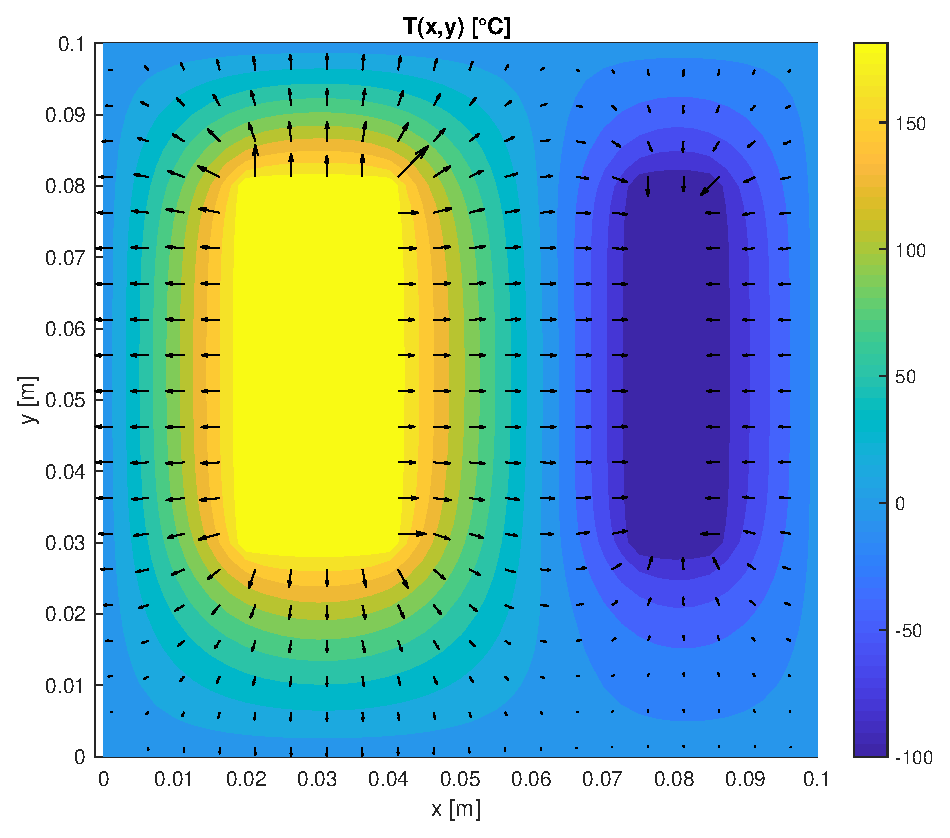
\includegraphics[width=\textwidth]{graphs/c_temp.eps}
%     \caption{Graph of temperatures, represented by the color gradient, in Kelvin, with the direction and the intensity of the heat flux represented by the arrows.}
%     \label{fig:c-temp}
%   \end{subfigure}
%   ~
%   \begin{subfigure}[t]{0.45\textwidth}
%     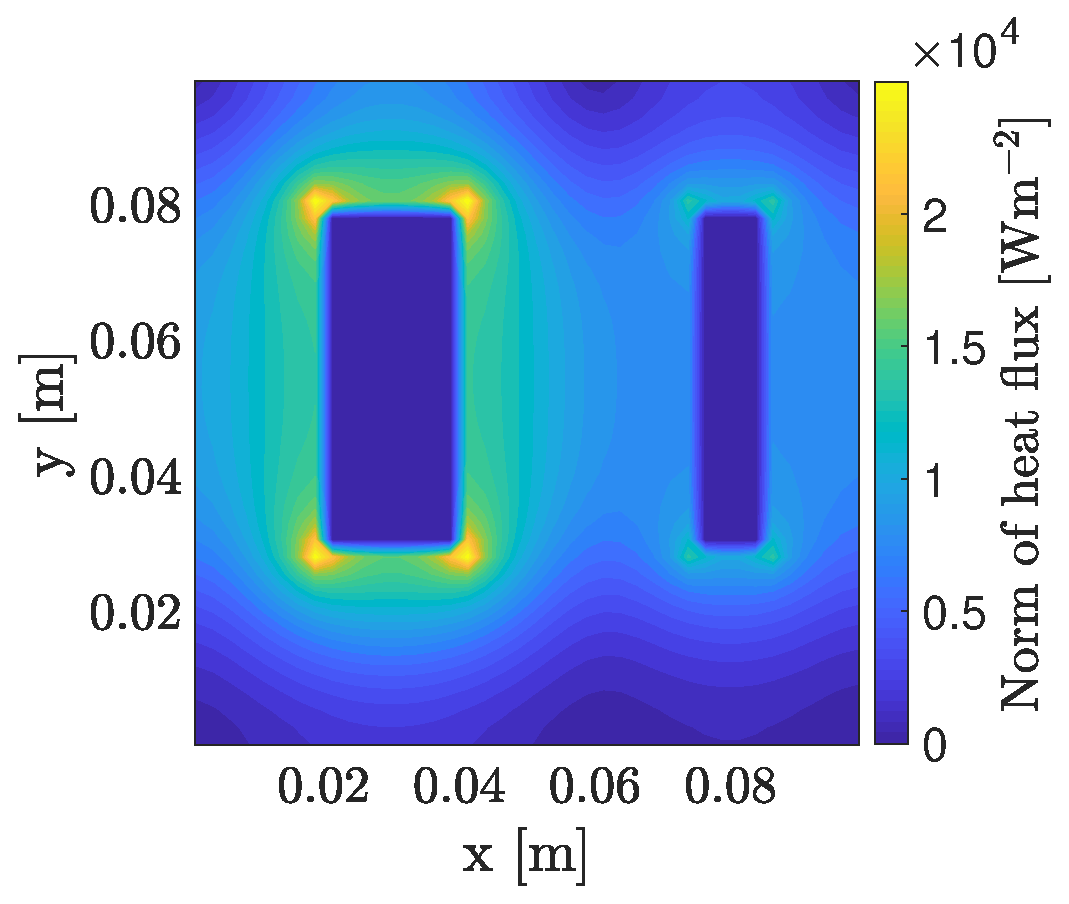
\includegraphics[width=\textwidth]{graphs/c_heat_flux.eps}
%     \caption{Intensity of the heat flux represented by the color gradient.}
%     \label{fig:c-heat-flux}
%   \end{subfigure}
%   \caption{Study of the heat flux at $t=\SI{0.1}{\second}$.}
%   \label{fig:c}
% \end{figure}

\section{Power study}
This section focuses on the study of the evolution of power emitted or received from both sources over time.
This power is measured using a closed surface, $S$ surrounding the zone of interest.
The power is defined by the surface integral stated by equation \eqref{eq:power}.

\begin{equation}
  P(t) = \iint_S \vec{j}(x,y,t)\cdot \text{d}\vec{\sigma}
  \label{eq:power}
\end{equation}

\paragraph{Numerical integration method.}
This first paragraph focuses on the method used to numerically integrate, and thus obtain the power.
Figure \ref{fig:d-mailles} is a diagram representing a simplified version of the mesh used in this project.
The crossings between the black lines are the temperature this point, the yellow square is the source considered, the blue circles are the horizontal heat flux $j_x$ obtained with a centered finite difference method on horizontal axis, the green circles are the vertical heat flux $j_y$ obtained with a centered finite difference method on vertical axis, vectors d$\vec{\sigma}$ are represented by the arrows and finally the red square is the Gauss surface $S$ considered.\\
%TODO : Je dis pas trop de la merde ?
To approximate the integral, it needs to be discretized.
A surface integral can be seen as a continuous sum over a surface $S$.
Thus, in a discrete modelisation, which is the case here, the surface integral can be replaced by a sum over several point.
It adds some uncertainties, but it is really easy to compute.
Thus, the power can be found by adding $\vec{j}_i\cdot d\vec{\sigma}$ for each point contained on the border of the surface $S$, where d$\vec{\sigma} = h\hat{e}_i$ with $h$ the distance between two nodes.
Note that $\vec{j}_i$ and $\hat{e}_j$ are either parallel or perpendicular, which means that the scalar product $\vec{j}_i\cdot\hat{e}_j$ is $\pm j_i$ when $i=j$ or $0$ when $i \neq j$.
%TODO : Expliquer comment a été calculée la puissance.

\begin{figure}[h]
  \centering
  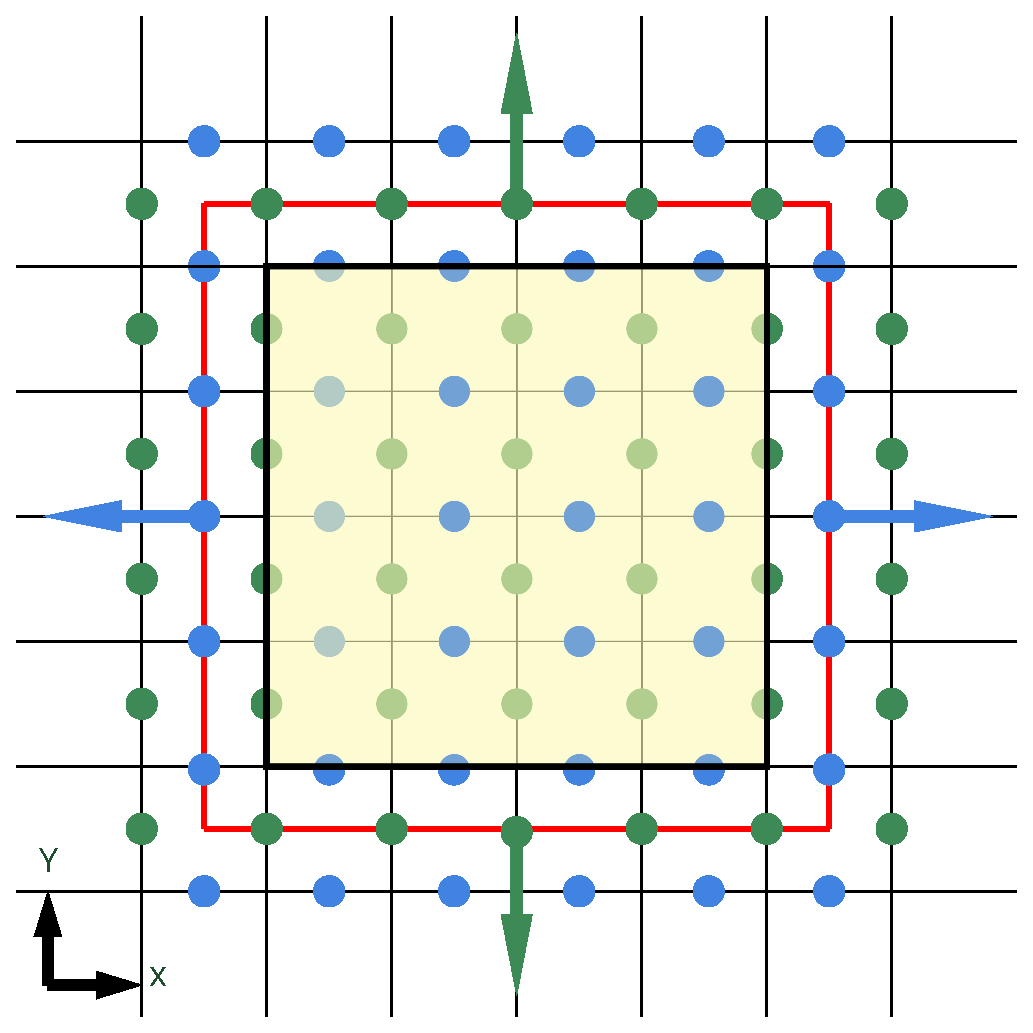
\includegraphics[width=0.5\textwidth]{graphs/d_mailles.eps}
  \caption{Mesh diagram considered in this project.}
  \label{fig:d-mailles}
\end{figure}

\paragraph{Analytical proof of surfaces equivalence.}
%TODO : Donner la preuve analytique que Pc + Pf = Ptot lorsque dT/dt -> 0.

\paragraph{Numerical evolution of power.}
This last paragraph focuses on the numerical results obtained by using the numerical method described earlier.
For a simulation of $t=\SI{0.5}{\s}$, the evolution of the power is available on figure \ref{fig:d-power}.

\begin{figure}[h]
  \centering
  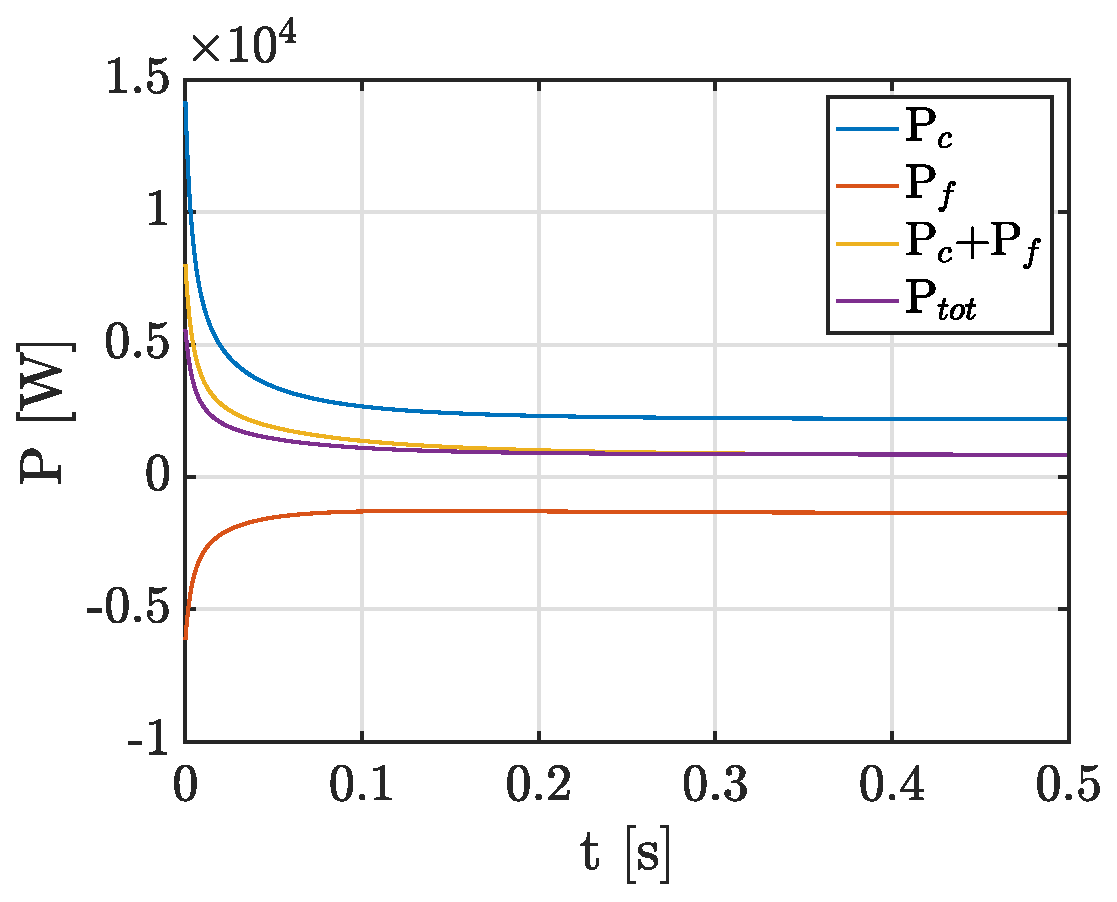
\includegraphics[width=0.6\textwidth]{graphs/d_power.eps}
  \caption{Evolution of power for \SI{0.5}{\s}.}
  \label{fig:d-power}
\end{figure}

The first information to notice on this figure is amplitude of power.
At the beginning, the power is of order \SI{10}{\kilo\watt}, which can seem really high.
And after a moment, the stabilized power is of order \SI{1}{\kilo\watt}.
This seems too much for a simple heat transfert between two small sources, but it may have multiple explaination.
In the first \num{25} milliseconds, the difference of temperature between the sources and the environment is not neglectable: $\Delta T=\SI{200}{\kelvin}$ for the hot source and $\Delta T=\SI{100}{\kelvin}$ for the cold source.
Thus, at the beginning, a hugh amount of heat is transfered in a short amount of time which is the reason why power is this high.
When the system is more stabilized, the difference is reduced, but still present.
As the sources are kept at their temperature, heat still flows from one to another with a difference of temperature of $\Delta T=\SI{300}{\kelvin}$.
This leads to a constant power emitted and received from the hot and the cold sources.\\

Another interesting point of this figure is that, after a long time (\SI{0.5}{\second} for example), the sum $P_c + P_f$, respectivelly the power emitted by the hot source and the power received by the cold source, is equal to the power measured with a surface surrounding both sources, $P_\text{tot}$.
Thus, as both curves seem to converge to the same power, the relation $\lim_{t\rightarrow\infty}P_c(t) + P_f(t) = \lim_{t\rightarrow\infty}P_\text{tot}(t)$ is verified.

\section{Temperature and heat flux with respect to the distance between the bodies}

In this section, the two bodies are brought closer together. To get an optimal curve, the halfway point between the two bodies (0.06,0.05) is chosen, and the bodies are displaced simultaneously closer together, by one grid unit at a time.

The results are displayed on Fig.\ref{fig:e}, where $\Delta x$ is the total displacement of one body. In other words, the distance between the two bodies at any point on the graph is $x_c-x_b-2\Delta x$. As the bodies are brought closer, the temperature at the halfway point, which is initially slightly higher than $0$°C, increases logarithmically up to $50$°C, which is the mean temperature of the two bodies $(T_c+T_f)/2$, before the hot body reaches it, at which point its temperature becomes $T_c=200$°C.

The norm of the stationary heat flux increases exponentially as the cold source and the hot source get closer. Indeed, the closer they are, the higher the norm of the saptial gradient of temperature is, as both extremes of temperature get farther from each other and more heat transfer occurs.

\begin{figure}[h]
  \centering
  \begin{subfigure}[t]{0.45\textwidth}
    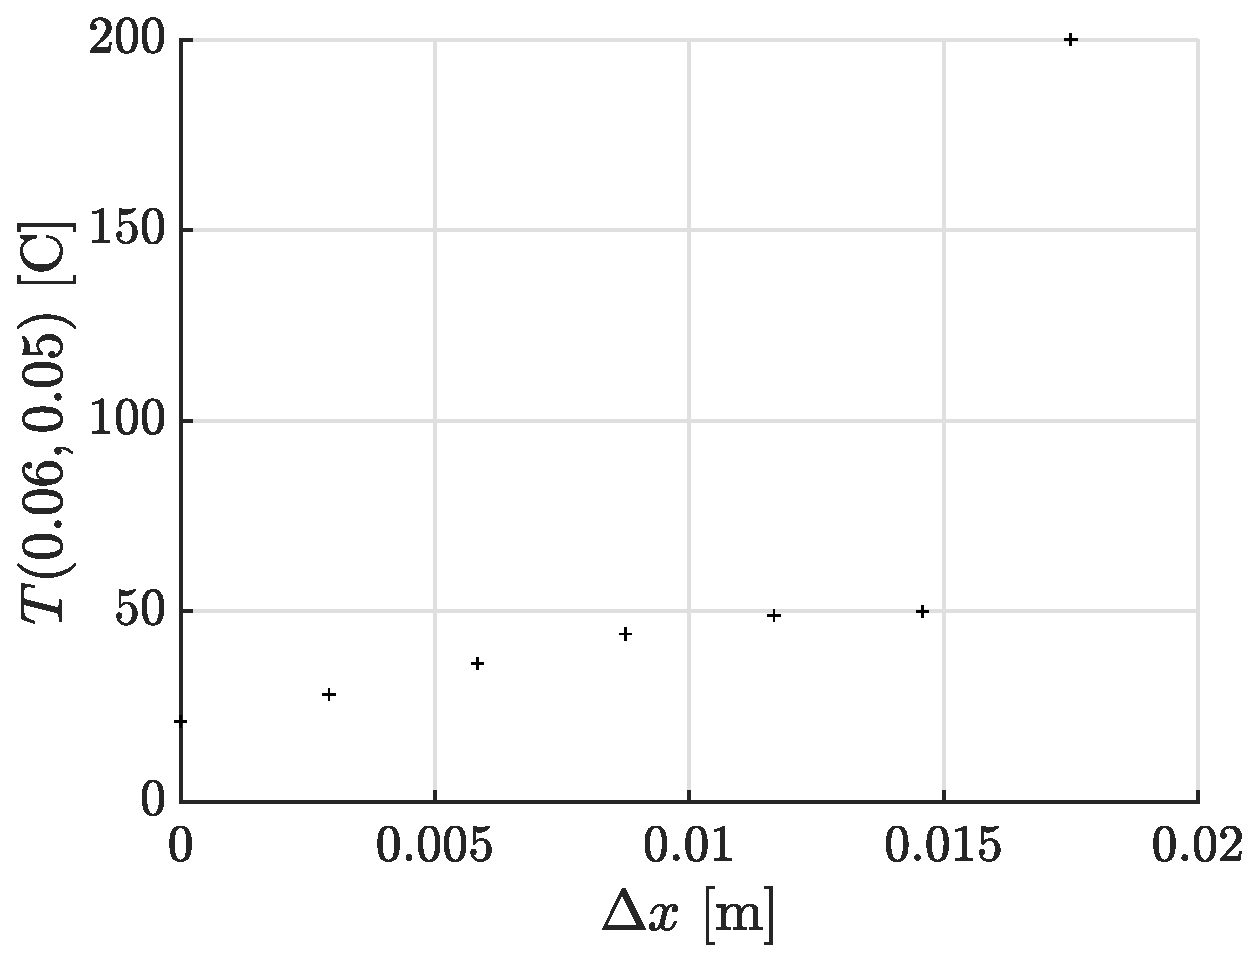
\includegraphics[width=\textwidth]{graphs/e_distT.eps}
    \caption{Temperature (in degrees Celsius)}
    \label{fig:e-T}
  \end{subfigure}
  ~
  \begin{subfigure}[t]{0.45\textwidth}
    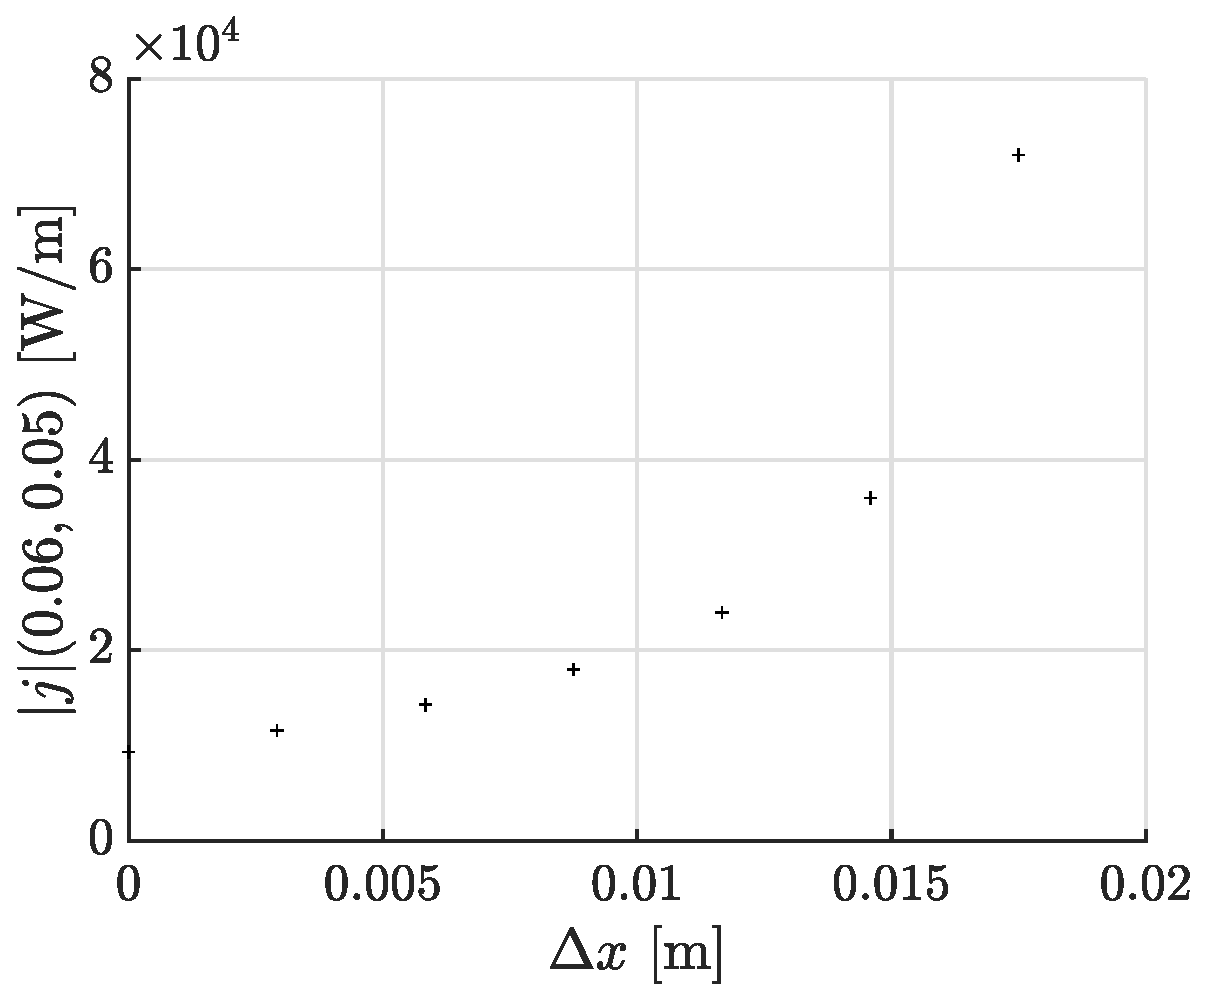
\includegraphics[width=\textwidth]{graphs/e_distF.eps}
    \caption{Heat flux}
    \label{fig:e-T}
  \end{subfigure}
  \caption{Temperature and heat flux in function of displacement}
  \label{fig:e}
\end{figure}

\section{Conclusion}

\begin{thebibliography}{99}
  \bibitem{wiki:2nd-law} Wikipedia contributors, "Second law of thermodynamics," Wikipedia, The Free Encyclopedia, \url{https://en.wikipedia.org/w/index.php?title=Second_law_of_thermodynamics&oldid=884867223} (accessed March 2, 2019).


\end{thebibliography}

\end{document}
